%TODO Armar seccion con los graficos 

\subsection{Análisis de corridas - Metodología}

Para poder analizar el comportamiento procesamos los archivos de log para las ejecuciones de los distintos modelos implementados en este trabajo.
El análisis de esta información fue realizado en distintos pasos.

Se tomó el archivo log base que indica qué archivo tiene la información de log para cada modelo.

Con esta información se generó un diccionario con la información de log desglozada para cada modelo y para cada tipo de evento. Los tipos de mensajes que categorizamos son los descriptos por Wainer. \ref{}

\begin{itemize}
    \item Los mensajes de tipo \textit{*} señalizan la ocurrencia de eventos internos.
    \item Los \textit{X} llevan información de la entrada de eventos externos.
    \item Los \textit{Y} transmiten los eventos de salida.
    \item Los mensajes \textit{done} llevan información de sincronización para futuros eventos, indicando que un modelo ha finalizado su tarea actual.
    \item Los mensajes  \textit{@} o también llamado mensaje de recolección,
        lleva señales para el simulador, indicandole que genere una salida.
    \item Los mensajes \textit{I} marcan la inicialización del modelo.
\end{itemize}

Buscamos analizar distintas variables. Por un lado las componentes
estructurales del modelo y por el otro, entender la evolución en el tiempo de
las salidas que arrojan los modelos.

\subsection{Análisis estructural}
Una estrategia para poder analizar la estructura del modelo es analizar la
cantidad de mensajes enviados por cada uno de sus componentes (modelos atómicos o acoplados). 
Esto nos permite ver los valores de salida emitidos por los modelo, de transiciones internas o eventos
externos.

Para un modelo sencillo como el de la taza de té generamos gráficos que nos
permiten analizar el comportamiento de la simulación en dos ejes, los eventos
realizados por cada atómico o el acoplado \texttt{top}.

Para poder generar este, categorizamos cada línea de log para cada modelo y
contamos su frecuencia. Luego, agrupamos estos datos y generamos un Heatmap.
Este gráfico nos permite visualizar las dimensiones \textit{modelo}, \textit{tipo de mensaje} y
\textit{cantidad de ocurrencias} para poder compararlos entre sí.

Dado que el \texttt{TopLevelCoupled} (TLC)  es el orquestador de la simulación,
observamos mayor cantidad de eventos de tipo \textit{@, Done e Y}. La alta
frecuencia de eventos \textit{Y} se explica sabiendo que éste  transporta la
información de salida. Dada la diferencia de magnitudes entre los distintos
modelos utilizamos una escala logarítmica y una escala lineal para analizar los
datos.

En la figura \ref{fig:teacup_cant_mensajes} observamos la  ejecución del modelo
de enfriamiento de una taza de té. En el eje de las $X$ tenemos los mensajes 
y en el eje de las $Y$ tenemos los distintos modelos. 
Esta figura se generó a partir de los datos simulados con el modelo traducido.
Podemos observar que para los modelos $FTot$, $FMinus$ e $Integrador$ la cantidad 
de transiciones internas, externas y de salida son iguales. Esto es razonable 
debido a que estos 3 modelos generan un ciclo entre sí, es decir que se retroalimentan.

Para poder analizar el comportamiento de las salidas de cada modelo, utilizamos
un gráfico de tipo LetterValue que puede observarse en \ref{fig:teacup_output_letter_plot}.
Éste nos indica además de los estadísticos principales (media, percentiles y outliers), 
la densidad de los valores que se encuentran en un rango de la muestra. 
Por ejemplo podemos ver que la muestra está no solo centrada en los 115 grados sino que 
más del 50\% de dichos valores se encuentran allí. 

En esta figura se observa claramente como los modelos de \textit{FTot} y \textit{FMinus} 
arrojan valores de out con un rango de valores acotado centrados alrededor del cero. 
En el caso del Integrador que es el que calcula los valores de temperatura de la taza, 
es razonable ver que los valores van desde los 180 grados a los 70. Se observa también 
la alta densidad de valores entre los 90 y los 135 grados. Los valores por debajo de los 
70 pueden tener que ver con el método de integración. 

Para mayor legibilidad quitamos los valores del modelo \textit{characteristictime} 
ya que este era constante y no aportaba al análisis.

\begin{figure}[H]
    \centering     %%% not \center
    \subfigure[Cantidad mensajes modelo teacup]{\label{fig:teacup_cant_mensajes}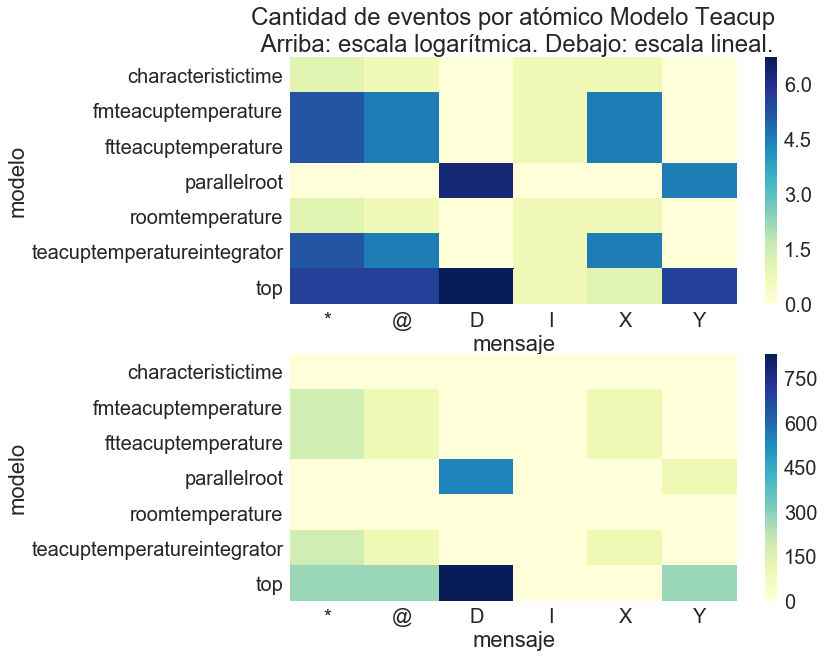
\includegraphics[scale=0.4]{imagenes/tea_cantidad_mensajes}}
        \subfigure[Valores de salida modelo teacup]{\label{fig:teacup_output_letter_plot}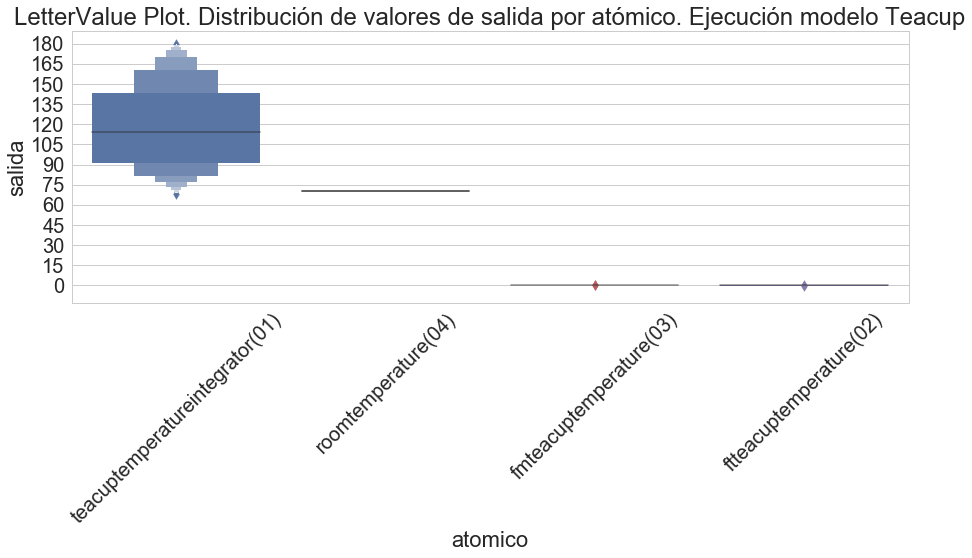
\includegraphics[scale=0.4]{imagenes/tea_output_letter_plot}}
        \caption{Modelo teacup - comportamiento estructural}
\end{figure}


Aplicamos la misma técnica para el análisis estructural del modelo SIR traducido.
En la figura \ref{fig:sir_cant_mensajes} podemos observar los distintos modelos
que interactúan en el modelo así como la cantidad de mensajes que envían por
cada tipo.
Por cómo está estructurado el modelo, se observa nuevamente que la cantidad de
mensaje de tipo \textit{*, @} coincide para los modelos relacionados con la
integración. 

\begin{figure}[H]
	\centering     %%% not \center
	\subfigure[Cantidad mensajes modelo SIR]{\label{fig:sir_cant_mensajes}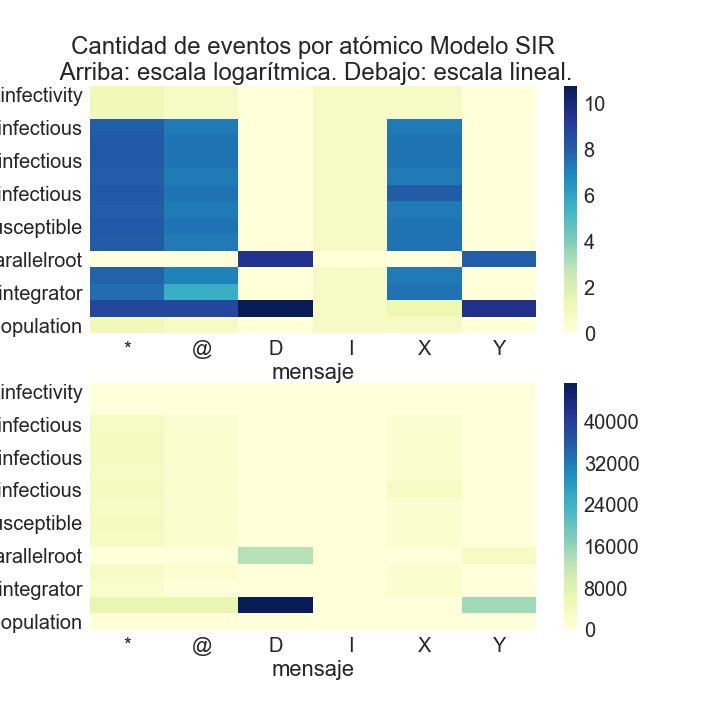
\includegraphics[scale=0.4]{imagenes/sir_cantidad_mensajes}}
	\subfigure[Valores de salida atómicos modelo SIR]{\label{fig:sir_output_letter_plot}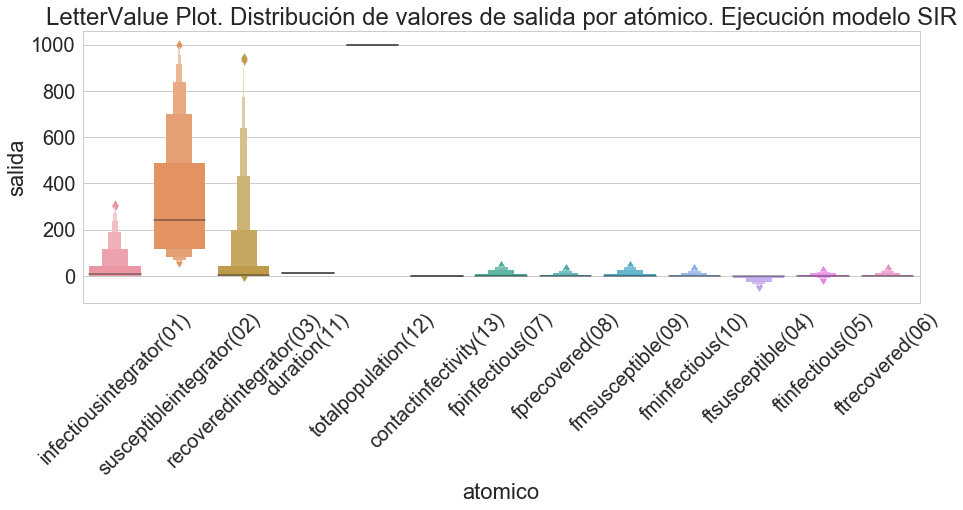
\includegraphics[scale=0.4]{imagenes/sir_output_letter_plot}}
        \caption{Modelo SIR - comportamiento estructural}
\end{figure}

\subsection{Análisis de los valores del modelo}

Para comparar los valores de las salidas entre el modelo traducido y el modelo
en \textit{SD} fue necesaria alinear la información para poder trabajar en las
mismas unidades de tiempo. Se puede ver un ejemplo en \ref{tab:times}. Por un lado los modelos de System Dynamics reportan
los valores de los Stocks en formato de punto flotante mientras que CD++
reporta la salida en formato fecha. Para llevar los a las mismas unidades,
decidimos llevar todo a segundos. Mantuvimos el formato en SD mientras que para las salidas de los modelos CD++ multiplicamos cada unidad de tiempo ( las horas y minutos) por la constante multiplicativa adecuada consiguiendo tener toda la información muestreada en segundos.

Reportamos los datos de la figura en un gráfico de tipo \textit{scatter} donde en el eje de las X se tienen los $t_i$ por cada medición para cada uno de los modelos.

\begin{table}[H]
    \centering
    \label{tab:times}
    \begin{tabular}{c | c  l}
        & Modelo SD & Modelo CD++ \\
       Datos originales & 121.125 & 00:02:01:125:0 \\ 
        Transformados & 121.125 & 121.125
    \end{tabular}
    \caption{Timestamps para los dos modelos} 
\end{table}


Observando la figura \ref{fig:teacup_salida_comparada} entendemos que hay diferencias en los comportamientos de los modelos. Por ejemplo, la tasa de decaimiento de la temperatura en el modelo traducido (en la figura valores en azul) nos muestra que la temperatura final se alcanza tres veces más rápido en CD++ que en SD.
También observamos que se alcanza el mismo valor final, motivo para pensar que la traducción funciona correctamente.

\begin{figure}[H]
    \centering     %%% not \center
	\subfigure[Comparación salida modelo teacup]{\label{fig:teacup_salida_comparada}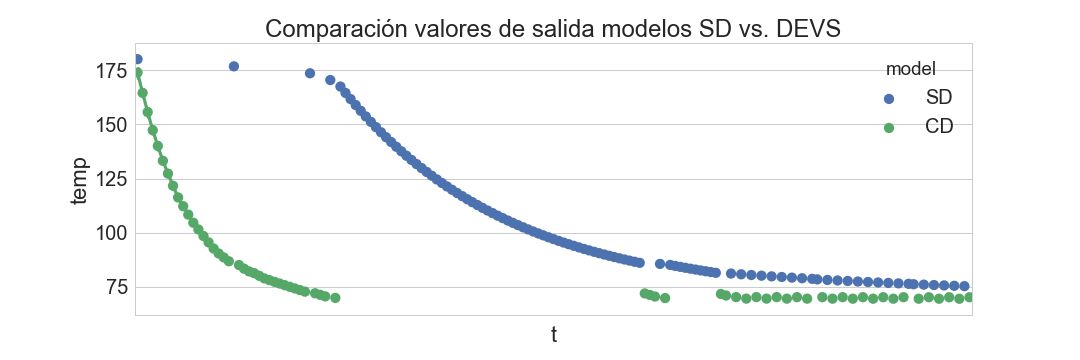
\includegraphics[scale=0.4]{imagenes/tea_comparada_salidas}}
\end{figure}

Si observamos en cambio la salida del modelo SIR observamos en las figuras \ref{fig:sir_infect}, \ref{fig:sir_recup} y \ref{fig:sir_sucep} que los valores coinciden en toda la evolución del sistema.

\begin{figure}[H]
    \centering     %%% not \center
    \subfigure[Comparación salida modelo SIR variable: Infectados]{\label{fig:sir_infect}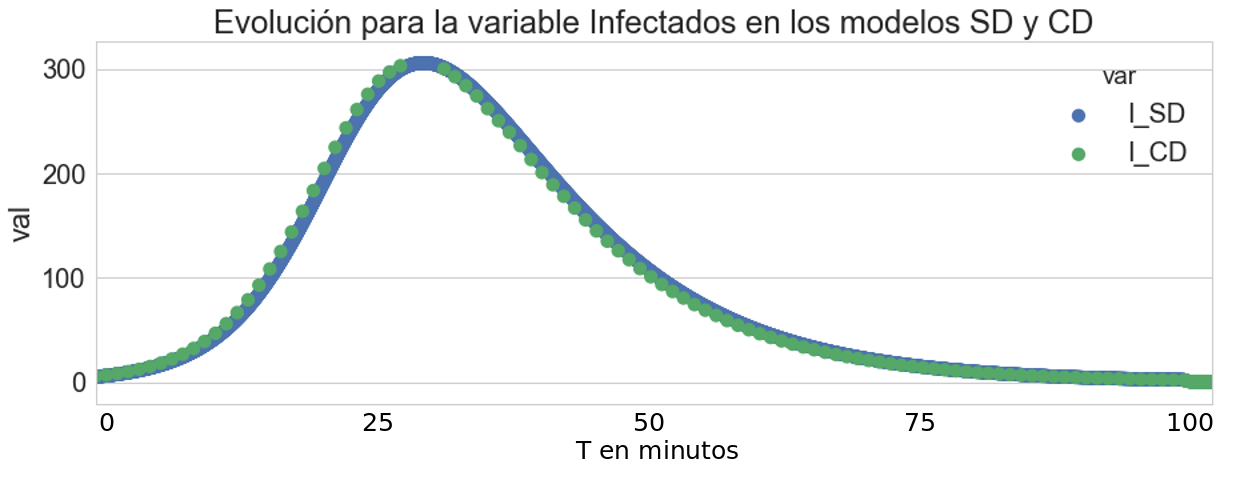
\includegraphics[scale=0.4]{imagenes/sir_comparada_salidas_infectados.png}}
    \subfigure[Comparación salida modelo SIR variable: Recuperandose]{\label{fig:sir_recup}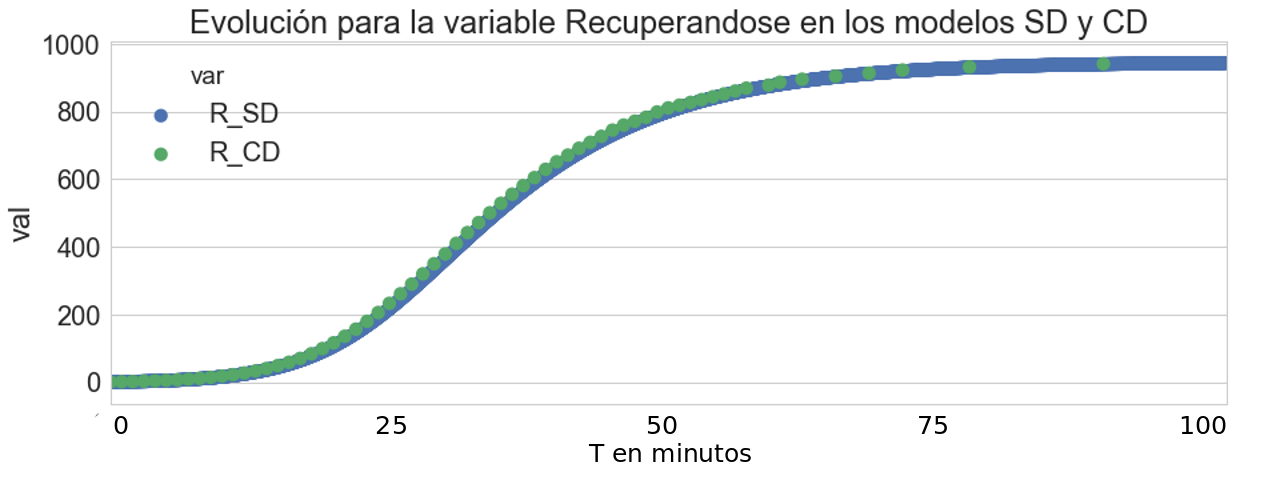
\includegraphics[scale=0.4]{imagenes/sir_comparada_salidas_recuperandose.png}}
    \subfigure[Comparación salida modelo SIR variable: Susceptibles]{\label{fig:sir_sucep}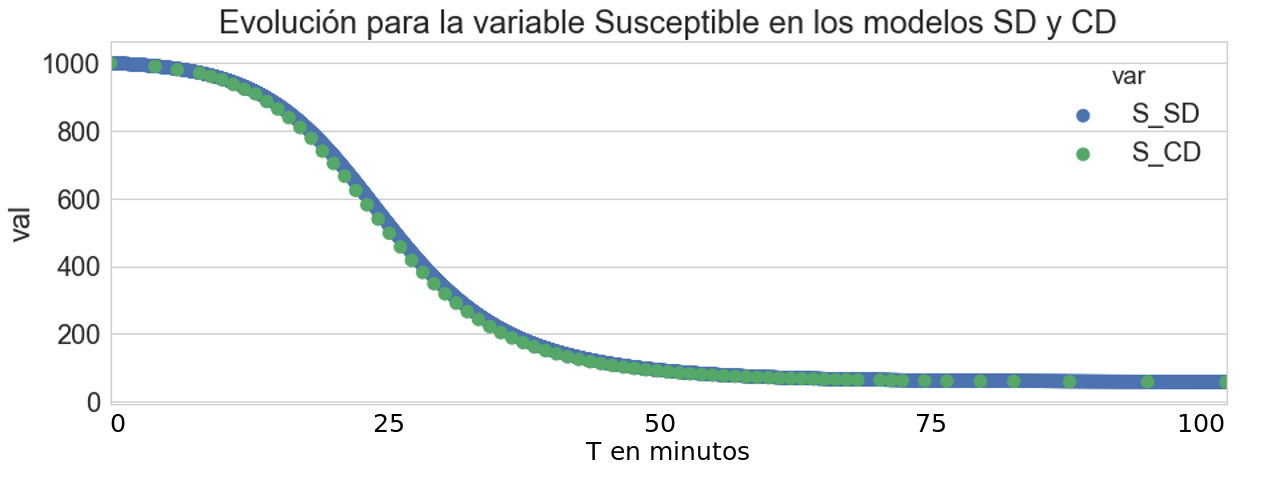
\includegraphics[scale=0.4]{imagenes/sir_comparada_salidas_suseptibles.png}}
        \caption{Modelo SIR - comparación de resultados}
\end{figure}

La granularidad de los dos modelos se explica ya que CD++ opera de manera discreta mientras que SD resuelve el sistema de manera continua.
